\chapter{Release experiment}\label{chap:release-experiment}
We released the MusicDAO system to a medium-scale network of 20+ mobile Android phones. We monitored the interactions between the devices during 7 days. 

We tested the viability of our DAO as a Big Tech alternative, by looking at three factors: scalability, content variety and longevity. Firstly, We investigated whether the latency of retrieving content is competitive in comparison to centralized alternatives. Secondly, we investigated how large a catalog of music can grow, in comparison to network size. Thirdly, we investigated the resiliency of content, meaning: to what extend backups are available of content. Lastly, we investigated the transfer speed of money to artists.

\section{Method}
To simulate a real-world situation, the MusicDAO system was evaluated by performing a release experiment. This means that participants were not supervised throughout the experiment. The approach to the experiment was as follows. Multiple Android users were invited to download and install MusicDAO. Consequently, they followed a step of tasks to complete within the app. While performing these tasks, all interaction data was recorded with timestamps, and saved on a remote server. After 7 days, this data was compiled for analysis.

During the 7-day release experiment, the network size is static. Every participant is asked to interact with a few pieces of music on each of these days. We measured the latency of various actions, and compared it to the catalog size. The catalog size is the total number of songs that are available in the network. To obtain expressive results in terms of scalability, we controlled the catalog size manually, and monitored the effect on the median latency. Every day, the catalog size was increased by X, starting with Y.

\section{Latency measurements}
Latency measurement results can be inspected in \ref{fig:buffering-performance} and \ref{fig:search-latency}.

\begin{figure}
    \centering
    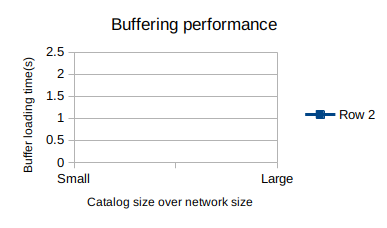
\includegraphics[width=0.5\textwidth]{experiments/buffering-performance.png}
    \caption{Buffering latency: the time between selecting a song and being able to stream it (without cache)}
    \label{fig:buffering-performance}
\end{figure}

\begin{figure}
    \centering
    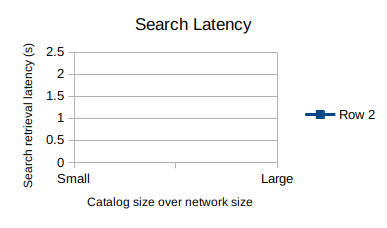
\includegraphics[width=0.5\textwidth]{experiments/search-latency.png}
    \caption{Search latency: the time between performing keyword search and retrieving results from a peer}
    \label{fig:search-latency}
\end{figure}

\section{Bootstrap measurements}
\ref{fig:content-discovery} shows the experience for first-time use of the application. When joining the network, a participant must discover other peers and download content metadata from them. The graph shows how much content can be browsed after a certain timespan. It is an evaluation of the peer discovery and bootstrap mechanisms.

\begin{figure}
    \centering
    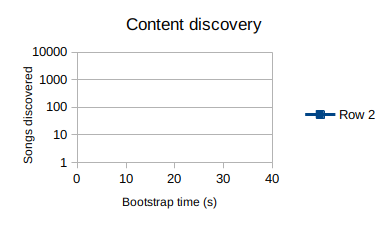
\includegraphics[width=0.5\textwidth]{experiments/content-discovery.png}
    \caption{Content discovery: the number of explored song metadata from starting the application and entering the network for the first time}
    \label{fig:content-discovery}
\end{figure}

\section{Resiliency measurements}
To measure the resiliency and longevity of published releases, we monitored its available duplicates after date of publishing. In other words, it shows how content penetrates through the network. The measurements shown in \ref{fig:content-discovery} are the duplicates of the track files. This can be viewed as a measurement of content availability.

\begin{figure}
    \centering
    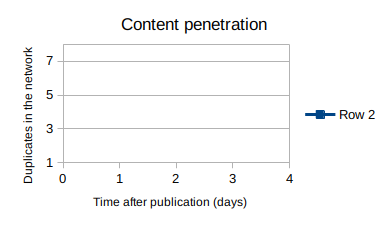
\includegraphics[width=0.5\textwidth]{experiments/content-penetration.png}
    \caption{Content penetration: from an artist perspective, how many backups there are available of the work that I published on the network}
    \label{fig:content-penetration}
\end{figure}

\section{Money transfer measurements}
We measured the latency of finalizing payments to artists, of which the results can be shown in table X.